%%%%%%%%%%%%%%%%%%%%%%%%%%%%%%%%%%%%%%%%%%%%%%%%%%%%%%%%%%%%%%%%%%%%%%%%%%%%%%%%%%%%%%%%%%%%%
%%									Chapitre 5												%
%%%%%%%%%%%%%%%%%%%%%%%%%%%%%%%%%%%%%%%%%%%%%%%%%%%%%%%%%%%%%%%%%%%%%%%%%%%%%%%%%%%%%%%%%%%%%

\chapter{Polynomial approximations for bivariate aggregate claims amount probability distributions}\label{Chapter5}
	\minitoc
	\newpage

%%%%%%%%%%%%%%%%%%%%%%%%%%%%%%%%%%%%%%%%%%%%%%%%%%%%%%%%%%%%%%%%%%%%%%%%%%%%%%%%%%%%%%%%%%%%%



% Début du chapitre

\begin{center}
\Large{\underline{\textbf{Abstract}}}\\
\end{center}
A numerical method to compute bivariate probability distributions from their Laplace transform is presented. The method consists in an orthogonal projection of the probability density function with respect to a probability measure that belongs to Natural Exponential Family with Quadratic Variance Function (NEF-QVF). The procedure allows a quick and accurate calculation of probabilities of interest and does not require strong coding skills. Numerical illustrations and comparisons with other methods are provided. This work is motivated by actuarial applications. We aim at recovering the joint distribution of two aggregate claims amount associated with two insurance policy portfolios that are closely related, and at computing survival functions for reinsurance losses in presence of two non-proportional reinsurance treaties.\\
\\
\textit{Keywords:} Bivariate aggregate claims model, bivariate distribution, bivariate
 Laplace transform, numerical inversion of Laplace transform, natural exponential families with quadratic variance functions, orthogonal polynomials.
\section{Introduction}
In insurance and in reinsurance, some common events may cause simultaneous, correlated claims in two lines of business. For example, in third-party liability motor insurance, an accident may cause corporal damage and material damage losses. These parts of the same claim are then handled by different claim managers and reserving is most often also done separately, which makes it necessary to study the joint distribution and not only the marginals or the distribution of the sum (except when one loss dominates the other one, which makes correlation of secondary importance). Similarly, a reinsurer who accepts two stop-loss treaties from two customers operating on the same market will be exposed to the sum of two excesses of aggregate losses, which contain in general some independent part and some common shock part, arising from events that generate claims for the two insurance companies at the same time. To compute the Value-at-Risk of the reinsurer's exposure, or to compute the probability that the reinsurer looses more than certain risk limits, we need the bivariate distribution of the aggregate claims amount of the two insurers. In addition to classical couples of independent aggregated losses drawn from compound distributions, one needs to study the common shock part of the bivariate loss vector.
We define a bivariate collective model with common shock by
\begin{equation}\label{ResinsuranceModelIntro}
\left( \begin{array}{l}
S_1 \\
S_2 \end{array}
\right)  =
 \displaystyle\sum_{j=1}^{N}
\left( \begin{array}{l}
U_{1j} \\
U_{2j} \end{array}
\right)
+
\left( \begin{array}{l}
X_{1} \\
X_{2} \end{array}
\right),
\end{equation}
where $(S_1, S_2)$ denote the aggregate claims amount of two non-life insurance portfolios over a given time period. The first part of the right-hand side of \eqref{ResinsuranceModelIntro} is the common shock part. A counting variable $N$ models the number of claims, and  $\{(U_{1j},U_{2j})\}_{j\in\mathbb{N}^{*}}$ is a sequence of \textbf{i.i.d} couples of non-negative random variables that model severities inccured in the two portfolios. We assume that the sequence $\{(U_{1j},U_{2j})\}_{j\in\mathbb{N}^{*}}$ is independent from $N$. We are interested in bivariate distributions that allow dependence between $U_{1j}$ and $U_{2j}$. The correlation between the claim amounts are related to the magnitude of the event causing the claims. The second part of the right-hand side of \eqref{ResinsuranceModelIntro} represents specific additional claim amounts that each insurer has to pay. The random vector $(X_{1},X_{2})$ is independent of the first part. The components are non-negative and mutually independent random variables. This modelization differs from what already exists in the literature. Correlation is usually specified upon the number of claims in two lines of business, see \citet{Am98,Am99}. Recursion based methods have been designed to cope with those kind of bivariate distributions, see \citet{Su99,Ve99}. Aggregate claims are governed by compound distributions. These distributions, in the univariate case, are already difficult to study because closed formulae for the probability density function are available in only a few cases. The cumbersome computation time induced by Monte Carlo simulations to obtain accurate values of probabilities motivates the use of numerical techniques.\\
In this paper, we develop an effective method to compute Bivariate Probability Density Functions (BPDFs) from the knowledge of their bivariate Laplace transform or equivalently from the moments of the distribution. First, we choose a reference distribution that belongs to a NEF-QVF. Then, we express the BPDF with respect to this reference measure as an expansion in terms of orthonormal polynomials. The polynomials are orthogonal with respect to the reference probability measure. When we aim at recovering a BPDF on the positive quadrant of the plane, as it is the case within the frame of aggregate claims amount distribution, our method looks like a well established method called the Laguerre method. The similarity is due to the fact that we choose a Gamma distribution as reference distribution associated with Laguerre polynomials to ensure the validity of the expansion. We refer to \citet{AbChWh95} where an effective variant of the Laguerre method is presented. The same authors also work out a multivariate extension, see \citet{AbChWh98}. The main contribution of our work lies in the possibility of choosing the parameters of the reference distribution to enhance the performance of the method. A great body of the applied probability literature is dedicated to the numerical inversion of the Laplace transform of univariate PDF but to the best of our knowledge only a few attempts have been made in a multivariate context. A Fourier series based method is presented in \citet{ChLuWh94} motivated by applications in queueing theory. The desired function is recovered from the Fourier series coefficients of a periodic version of the function constructed by aliasing. The inversion formula involves integral computations that are completed using a trapezoidal rule justified by Poisson summation formula. It also implies truncation but not a simple one: Euler summation formula for alternating series is employed consequently to the neat replacement of the original infinite serie by an equivalent alternating one. Interesting applications are allowed because of the possibility of recovering MPDFs of couples of random variables formed by a discrete and a continuous one. We want to mention the work of Jin and Ren \citet{JiRe13}. A model very similar to the one defined in \ref{ResinsuranceModelIntro} is considered and a comparison between Fourier series and recursion based method is performed. Recently, a moment-recovered approximation has been proposed in \citet{Mn11}. The stable approximants for the BPDF and the joint survival function is derived. A very interesting feature of this method is that the approximation can turned into a statistical estimation as there exist empirical counterparts of the aforementioned approximants. The expansion we propose is also well adapted to empirical estimation. The empirical estimation of BPDF when data are available will be at the center of a forthcoming paper. Finally, one key aspect of the method is that once the parameters has been choosen and the coefficients computed, approximations for the joint probability density and survival functions are available in an explicit form.\\
In Section 2, we introduce a BPDF expansion formula based on orthogonal projection within the frame of NEF-QVF. In Section 3, the expansion for bivariate aggregate claims amount distributions is derived along with conditions to ensure the validity of the polynomial expansion. Section 4 is devoted to numerical illustrations and examples of application. A comparison to the moment-recovered method is also proposed. 
\section{Expression of the joint density}
\subsection{Orthogonal polynomials associated with NEF-QVF}
Let $F=\{F_{\theta},\theta\in\Theta\}$ with $\Theta\subset \mathbb{R}$ be a Natural Exponential Family (NEF), see \citet{Ba78}, generated by a probability measure $\nu$ on $\mathbb{R}$ such that
\begin{eqnarray*}
F_{\theta}(X\in A)&=&\int_{A}exp\{x\theta-\kappa(\theta)\}d\nu(x)\\
&=&\int_{A}f(x,\theta)d\nu(x),
\end{eqnarray*}
where $A\subset\mathbb{R}$, $\kappa(\theta)=log\left(\int_{\mathbb{R}}e^{\theta x}d\nu(x)\right)$ is the Cumulant Generating Function (CGF), and $f(x,\theta)$ is the density of $P_{\theta}$ with respect to $\nu$.
Let $X$ be a random variable  $F_{\theta}$ distributed. The mean of $X$ is
\[
m=E_{\theta}(X)=\int xdF_{\theta}(x)=\kappa'(\theta),
\]
and its variance is
\begin{equation*}
V(m)=Var_{\theta}(X)=\int (x-m)^{2}dF_{\theta}(x)=\kappa''(\theta).
\label{Variance}
\end{equation*}
The application $\theta\rightarrow\kappa'(\theta)$ is one to one. Its inverse function $m\rightarrow h(m)$ is defined on $\cal{M}$ $=\kappa'(\Theta)$. With a slight change of notation, we can rewrite $F=\{F_{m},m \in\cal{M}\}$, where $F_{m}$ has mean $m$ and density $f(x,m)=exp\{h(m)x-\kappa(h(m))\}$ with respect to $\nu$. A NEF has a Quadratic Variance Function (QVF) if there exist reals $v_0, v_1, v_2$ such that 
\begin{equation}\label{QVF}
V(m)=v_{0}+v_{1}m+v_{2}m^{2}.
\end{equation}
The Natural Exponential Families with Quadratic Variance Function (NEF-QVF) include the normal, gamma, hyperbolic, Poisson, binomial and negative binomial distributions.\\
Define
\begin{equation}\label{Poly1}
P_{k}(x,m)=V^{n}(m)\left\{\frac{\partial^{n}}{\partial m^{n}}f(x,m)\right\}/f(x,m),
\end{equation}
for $n\in\mathbb{N}$. Each $P_{n}(x,m)$ is a polynomial of degree $n$ in both $m$ and $x$. Moreover, if F is NEF-QVF, $\{P_{n}\}_{n\in\mathbb{N}}$ is a family of orthogonal polynomials with respect to $P_{m}$ in the sense that
\[
<P_{k},P_{l}>=\int P_{k}(x,m)P_{l}(x,m)dF_{m}(x)=\delta_{kl}||P_{k}||^{2},\hspace{1cm}k,l\in\mathbb{N},
\]
where $\delta_{kl}$ is the Kronecker symbol equal to $1$ if $k=l$ and $0$ otherwise. For the sake of simplicity, we choose $\nu=F_{m_{0}}$. Then, $f(x,m_{0})=1$ and we write
\begin{equation}\label{Poly2}
P_{k}(x)=P_{k}(x,m_{0})=V^{k}(m_{0})\left\{\frac{\partial^{k}}{\partial m^{k}}f(x,m)\right\}_{m=m_{0}}.
\end{equation}
We also consider in the rest of the paper a normalized version of the polynomials defined in \eqref{Poly2} with $Q_{k}(x)=\frac{P_{k}(x)}{||P_{k}||}$. For an exhaustive review regarding NEF-QVF and their properties, we refer to \citet{Mo82}.
\subsection{Bivariate probability measures and their Laplace transform}
Let $(X,Y)$ be a couple of random variables, governed by a bivariate probability measure $F_{X,Y}$. We also assume that $(X,Y)$ admits a joint probability density function with respect to a bivariate measure denoted by $\lambda$, such that 
\begin{equation}\label{BivariateProbabilityMeasure}
dF_{X,Y}(x,y)=f_{X,Y}(x,y)d\lambda(x,y).
\end{equation} 
Its bivariate Laplace transform is defined as
\begin{equation}\label{BivariateLaplaceTransform}
\widehat{f_{X,Y}}(s,t)=\int\int e^{sx+ty}f_{X,Y}(x,y)d\lambda(x,y).
\end{equation}
We consider the bivariate NEF-QVF generated by
\begin{equation}\label{NEFQVFBivariateMeasure}
d\nu(x,y)=d\nu_{1}(x)\times d\nu_{2}(y),
\end{equation}
where $\nu_{1}$ and $\nu_{2}$ are two probability measures that belong to NEF-QVF absolutely continuous with respect to $\lambda$. With the notation of Section 2.1, the probability density function associated with $\nu$ is 
\begin{equation}\label{BivariateNEFQVFPDF}
f(x,y)=f(x,m_{1})f(y,m_{2}).
\end{equation}
Let $Q_{k,l}(x,y)=Q_{k}^{1}(x)Q_{l}^{2}(y)$ be a bivariate polynomial system that is orthogonal with respect to $\nu$. We have
\begin{eqnarray*}
<Q_{k,l},Q_{i,j}>&=&\int\int Q_{k,l}(x,y)Q_{i,j}(x,y)d\nu(x,y)\\
<Q_{k,l},Q_{i,j}>&=&\delta_{ki}\delta_{lj}.
\end{eqnarray*}
We denote by $L_{2}(\nu)$ the set of functions square integrable with respect to $\nu$.
\begin{Prop}\label{BivariateDensityExpansionTheo1}
Assume that $\frac{dF_{X,Y}}{d\nu}\in L_{2}(\nu)$, we have the following expansion
\begin{eqnarray}
\frac{dF_{X,Y}}{d\nu}(x,y)&=&\sum_{k=0}^{+\infty}\sum_{l=0}^{+\infty}<\frac{dF_{X,Y}}{d\nu},Q_{k,l}>Q_{k,l}(x,y)\\
&=&\sum_{k=0}^{+\infty}\sum_{l=0}^{+\infty}E(Q_{k,l}(X,Y))Q_{k,l}(x,y).
\end{eqnarray}
\end{Prop}
Applying Proposition \ref{BivariateDensityExpansionTheo1} yields an expansion of the probability density function
\begin{equation}\label{BivariateDensityExpansion2}
f_{X,Y}(x,y)=\sum_{k=0}^{+\infty}\sum_{l=0}^{+\infty}\int\int \left(f_{X,Y}(x,y)Q_{k,l}(x,y)dxdy\right)\times Q_{k,l}(x,y)f(x,y).
\end{equation}
We have
\begin{equation}\label{BivariatePolynomial}
Q_{k,l}(x,y)=\sum_{i=0}^{k}\sum_{j=0}^{l}q_{i,j}(k,l)x^{i}y^{j},
\end{equation}
 where $q_{i,j}(k,l)$ is expressed in terms of the coefficents of $Q_{k}^{1}$ and $Q_{l}^{2}$. Reinjecting the expression of $Q_{k,l}$ given in \eqref{BivariatePolynomial} in the probability density function \eqref{BivariateDensityExpansion2} gives the two following representations of $f_{X,Y}$
\begin{eqnarray}\label{BivariateDensityExpansion3}
f_{X,Y}(x,y)&=&\sum_{k=0}^{+\infty}\sum_{l=0}^{+\infty}\sum_{i=0}^{k}\sum_{j=0}^{l}q_{i,j}(k,l)\int\int x^{i}y^{j}f_{X,Y}(x,y)dxdy\times Q_{k,l}(x,y)f(x,y)\nonumber\\
&=&\sum_{k=0}^{+\infty}\sum_{l=0}^{+\infty}\sum_{i=0}^{k}\sum_{j=0}^{l}q_{i,j}(k,l)\left[\frac{\partial^{i+j}}{\partial s^{i}\partial t^{j}}\widehat{f_{X,Y}}(s,t)\right]_{s=0,t=0}Q_{k,l}(x,y)f(x,y)\nonumber\\
&\doteq&\sum_{k=0}^{+\infty}\sum_{l=0}^{+\infty}a_{k,l} Q_{k,l}(x,y)f(x,y).\nonumber
\end{eqnarray}
\begin{Rk}
The probability density function takes the form of an expansion. The coefficients are expressed in terms of the moments and equivalently in terms of the derivative of the bivariate Laplace transform. The expression of the probability density function is therefore a Laplace transform inversion formula.
\end{Rk}
Approximation of the bivariate probability density function is obtained through truncation of the infinite series
\begin{equation}
f^{K,L}_{X,Y}(x,y)=\sum_{k=0}^{K}\sum_{l=0}^{L}a_{k,l} Q_{k,l}(x,y)f(x,y)\nonumber,
\end{equation}
where $K$ and $L$ denote the order of truncation of the approximation. In view of future applications, we are interested in getting approximations of cumulative distribution functions, which are obtained through integration of the approximated density
\begin{eqnarray}
F_{X,Y}^{K,L}(x,y)&=&\int_{-\infty}^{x}\int_{-\infty}^{y}f^{K,L}_{X,Y}(u,v)d\lambda(u,v)\\
&=&\sum_{k=0}^{K}\sum_{l=0}^{L}a_{k,l}\int_{-\infty}^{x}\int_{-\infty}^{y} Q_{k,l}(u,v)f(u,v)d\lambda(u,v).
\end{eqnarray}
The goodness of the approximation lies in the decay of the sequence defined by the coefficients of the expansion. Note that from $\frac{dF_{X,Y}}{d\nu}\in L_{2}(\nu)$, a Parseval type relation holds
\begin{equation}\label{ParsevalRelation}
\int\int f_{X,Y}^{2}(x,y)dxdy = \sum_{k=0}^{+\infty}\sum_{l=0}^{+\infty}a_{k,l}^{2}<+\infty.
\end{equation}
Relation \eqref{ParsevalRelation} implies that the sequence $\{a_{k,l}\}_{k,l\in\mathbb{N}}$ decreases towards 0 with respect to $k$ and $l$. The choice of the NEF-QVF and its parameters depends on the problem, and are discussed in the next section.
\section{Application to a bivariate aggregate claims amount distribution}
\subsection{General formula}
Aggregate claims amount are modeled by non-negative random variables. The only NEF-QVF with support on $\mathbb{R}^{+}$ is generated by the Gamma distribution that admits a probability density function with respect to the Lebesgue measure defined as 
\begin{equation}\label{GammaPDF}
f(x)=\frac{x^{r-1}e^{-x/m}}{\Gamma(r)m^{r}}.
\end{equation}
The orthogonal polynomials associated with the Gamma distribution are the generalized Laguerre polynomials
\begin{equation}\label{LaguerrePolynomials}
Q_{k}(x)=\frac{(-1)^{k}L_{k}^{r-1}(x/m)}{\sqrt{\binom{k+r-1}{k}}},
\end{equation}
where $L_{n}^{r-1}(x)=\sum^{n}_{i=0}\binom{n+r-1}{n-i}\frac{(-x)^{i}}{i!}$, see \citet{Sz39}. The random couple $(S_{1},S_{2})$, defined in \eqref{ResinsuranceModelIntro}, is divided into two parts. We denote by 
 \begin{equation}\label{BivariateCompoundDistributionRV}
\left( \begin{array}{l}
Y_1 \\
Y_2 \end{array}
\right)  =
 \displaystyle\sum_{j=1}^{N}
\left( \begin{array}{l}
U_{1j} \\
U_{2j} \end{array}
\right)
\end{equation}
the first part which is governed by a bivariate compound distribution. The study of the distribution of $(X_{1},X_{2})$ may be reduced to univariate problem that we can easily handle due to the independence of the components. The distribution of $(Y_{1},Y_{2})$ is unknown and we apply polynomial expansion in order to recover its BPDF. The BPDF of $(S_{1},S_{2})$ is obtained using a two-dimensional convolution procedure. The bivariate probability measure associated with $(Y_{1},Y_{2})$ is divided into a discrete part with an atom at $(0,0)$ with a probability mass equal to $p_{0}=P(N=0)$ and a continuous part that is absolutely continuous with respect to the bivariate Lebesgue measure
\begin{equation}\label{BivariateAgregateClaimProbabilityMeasure}
dF_{Y_{1},Y_{2}}(x,y)=p_{0}\delta_{\{x=0,y=0\}}(x,y)+dG_{Y_{1},Y_{2}}(x,y),
\end{equation}
where $\delta_{\{x=0,y=0\}}(x,y)$ is the Dirac measure equal to $1$ at $(0,0)$ and $0$ otherwise. We aim at expanding the continuous part using Proposition \ref{BivariateDensityExpansionTheo1}. The defective density probability function of $dG_{Y_{1},Y_{2}}$ is denoted by $g_{Y_{1},Y_{2}}$. We define a bivariate NEF-QVF probability measure as in Section $2$ by
\begin{equation}
\nu(x,y)=\nu_{1}(x)\times\nu_{2}(y),
\end{equation}
where $\nu_{1}$ and $\nu_{2}$ are Gamma distributions with parameter $(m_{1},r_{1})$ and $(m_{2},r_{2})$ respectively. Orthogonal polynomials with respect to $\nu$ are defined by 
\begin{equation}
Q_{l,k}(x,y)=Q^{1}_{k}(x)\times Q^{2}_{l}(y),
\end{equation}
where $\{Q^{1}_{k}\}_{k\in\mathbb{N}}$ and $\{Q^{2}_{l}\}_{l\in\mathbb{N}}$ are orthogonal polynomial systems with respect to $\nu_{1}$ and $\nu_{2}$ respectively, and defined as in \eqref{LaguerrePolynomials}. If $\frac{dG_{Y_{1},Y_{2}}}{d\nu}\in L^{2}(\nu)$, applying Proposition \ref{BivariateDensityExpansionTheo1} yields
\begin{equation}\label{DefectiveDensityExpansion}
g_{Y_{1},Y_{2}}(x,y)=\sum_{k=0}^{+\infty}\sum_{l=0}^{+\infty}a_{k,l} Q_{k,l}(x,y)f_{\nu}(x,y),
\end{equation} 
where $f$ is the BPDF associated to the probability measure $\nu$.
\begin{Rk}
The Laguerre series method in \citet{AbChWh98} is related to our approach with a particular parametrization that is $m_{1}=m_{2}=2$ and $r_{1}=r_{2}=1$.
\end{Rk}
We know from the Parseval type relation \eqref{ParsevalRelation} that the sequence of coefficients of the expansion is decreasing towards $0$. But how fast does it actually decrease?\\
We address this problem using generating function theory just like what is done in \citet{AbChWh98}. The interesting fact is that the generating function of the coefficients of the expansion is linked to the bivariate Laplace transform of the expanded probability density function. We start from the expression given in \eqref{DefectiveDensityExpansion}. By taking the bivariate Laplace transform we get
\begin{eqnarray}\label{LaplaceTransformToGenFunction}
\widehat{g_{Y_{1},Y_{2}}}(s_{1},s_{2})&=&\int_{0}^{+\infty}\int_{0}^{+\infty}e^{s_{1}x+s_{2}y}g_{Y_{1},Y_{2}}(x,y)
dxdy\nonumber\\
&=&\sum_{k=0}^{+\infty}\sum_{l=0}^{+\infty}a_{k,l}
(-1)^{k+l}\sqrt{\binom{k+r_{1}-1}{k}\binom{l+r_{2}-1}{l}}\nonumber\\
&\times&\left(\frac{1}{1-s_{1}m_{1}}\right)^{r_{1}}\left(\frac{1}{1-s_{2}m_{2}}\right)^{r_{2}}\left(\frac{s_{1}m_{1}}{s_{1}m_{1}-1}\right)^{k}\left(\frac{s_{2}m_{2}}{s_{2}m_{2}-1}\right)^{l}\nonumber\\
&=&\left(\frac{1}{1-s_{1}m_{1}}\right)^{r_{1}}\left(\frac{1}{1-s_{2}m_{2}}\right)^{r_{2}}B\left(\frac{s_{1}m_{1}}{s_{1}m_{1}-1},\frac{s_{2}m_{2}}{s_{2}m_{2}-1}\right),
\end{eqnarray}
where
\begin{equation}\label{CoefficientGeneratingFunction}
B(z_{1},z_{2})=\sum_{k=0}^{+\infty}\sum_{l=0}^{+\infty}b_{k,l}z_{1}^{k}z_{2}^{l}
\end{equation}
is the generating function of the two-dimensional sequence $\{b_{k,l}\}_{k,l\in\mathbb{N}}$. The coefficients of the expansion follow from 
\begin{equation}
a_{k,l}=b_{k,l}\frac{(-1)^{k+l}}{\sqrt{\binom{k+r_{1}-1}{k}\binom{l+r_{2}-1}{l}}}.
\end{equation}
The generating function $B$ is derived from the Bivariate Laplace transform after a simple change of variable in Equation \eqref{LaplaceTransformToGenFunction}:
\begin{equation}\label{GenFunctionToLaplaceTransform}
B(z_{1},z_{2})=(1-z_{1})^{-r_{1}}(1-z_{2})^{-r_{2}}\widehat{g_{Y_{1},Y_{2}}}\left(\frac{z_{1}}{m_{1}(1-z_{1})},\frac{z_{2}}{m_{2}(1-z_{2})}\right).
\end{equation} 
In \citet{AbChWh98}, the authors compute the coefficients of the expansion through the derivative of their generating function. They use Cauchy contour integral to express the derivatives as integrals and  approximate them via a trapezoidal rule. In some cases, when the Laplace transform expression is simple, the derivatives can be calculated directly with a computational software . The attractive feature of our method lies in the possibility of tuning the parameters of the Gamma distributions in order to modify the generating function. We illustrate this fact through the following example:
\begin{Ex}
Let $(X,Y)$ be a couple of independent random variables exponentially distributed with parameters $\delta_{1}$ and $\delta_{2}$. The bivariate Laplace transform associated with this couple of random variables is 
\begin{equation}\label{BivariateLaplaceTransformIndependantExponentialRV}
\widehat{f_{X,Y}}(s_{1},s_{2})=\frac{\delta_{1}}{\delta_{1}-s_{1}}\times\frac{\delta_{2}}{\delta_{2}-s_{2}}.
\end{equation}
We inject the bivariate Laplace transform expression \eqref{BivariateLaplaceTransformIndependantExponentialRV} in the generating function defined in \eqref{GenFunctionToLaplaceTransform} to get
\begin{equation}\label{CoefficientGeneratingFunctionIndependantExponentialRV}
B(z_{1},z_{2})=\frac{(1-z_{1})(1-z_{2})}{(1-z_{1})^{r_{1}}(1-z_{2})^{r_{2}}}\times\frac{\delta_{1}\delta_{2}}{\left[\delta_{1}+z_{1}(1/m_{1}-\delta_{1})\right]\left[\delta_{2}+z_{2}(1/m_{2}-\delta_{2})\right]}.
\end{equation}
In this case, the parametrization is straightforward. We set $r_{1}=r_{2}=1$, $m_{1}=1/\delta_{1}$ and $m_{2}=1/\delta_{2}$, so $B(z_{1},z_{2})=1$ which implies that $a_{0,0}=1$ and $a_{k,l}=0$ for all $k,l\geq1$.
\end{Ex} 
The Laplace transform of the distributions that we consider in the rest of the paper is more complicated and it is less straightforward to choose the parameters. In the next Section, we show how to choose the parameters of the expansion in order to ensure the integrability condition on Proposition \ref{BivariateDensityExpansionTheo1}.
\subsection{Integrability condition}
The polynomial expansion is valid under the following condition: 
\begin{equation}\label{Integrabilitycondition1}
\int_{0}^{+\infty}\int_{0}^{+\infty}\left(\frac{dG_{Y_{1},Y_{2}}}{d\nu}(x,y)\right)^{2}d\nu(x,y)<+\infty,
\end{equation}
which is equivalent to 
\begin{equation}\label{Integrabilitycondition2}
\int_{0}^{+\infty}\int_{0}^{+\infty}g_{Y_{1},Y_{2}}(x,y)^{2}x^{1-r_{1}}y^{1-r_{2}}e^{x/m_{1}+y/m_{2}}dxdy<+\infty.
\end{equation}
The parameters $m_{1}$, $m_{2}$, $r_{1}$ and $r_{2}$ of the reference distribution have a key role regarding the validity of the polynomial expansion. We define the set
\begin{equation}
E=\{(s,t)\in[0,+\infty)\times [0,+\infty) ; \widehat{f}(s,t)<+\infty\},
\end{equation}
and denote by $E^{c}$ its complementary. The following result gives us insight on how to choose the parameters of the reference distribution.
\begin{Theo}\label{IntegrabiltyConditionVersion2}
Let $(X,Y)$ be a couple of non-negative random variables with a joint PDF $f(x,y)$. We assume that $E\neq\{(0,0)\}$. We assume additionally that there exist two real numbers $a, b\geq0$ such that for all $(x,y)\in[a,+\infty) \times [b,+\infty)$, the applications $x\rightarrow f(x,y)$ and $y\rightarrow f(x,y)$ are strictly decreasing. Then we have 
\begin{equation}\label{FatInequality}
f(x,y)\leq A(s,t)e^{-sx-ty}, \hspace{0.1cm} \forall (x,y)\in[a,+\infty) \times [b,+\infty),
\end{equation} 
where $A(s,t)$ is some real number independent of $x$ and $y$.
\end{Theo}
\begin{proof}
Let $(x,y)\in[a,+\infty) \times [b,+\infty)$, we have 
\begin{eqnarray}
\widehat{f}(s,t)&>&\int_{a}^{x}\int_{b}^{y}e^{su+tv}f(u,v)dudv\nonumber\\
&=&\int_{a}^{x}e^{su} \frac{1}{t}(e^{tv}f_{X,Y}(u,y)-e^{tb}f(u,b))dudv\nonumber\\
&-&\int_{a}^{x}e^{su}\int_{b}^{y}\frac{e^{tv}}{t}\frac{\partial f(u,v)}{\partial v}dudv\nonumber\\
&>&\int_{a}^{x}e^{su} \frac{1}{t}(e^{tv}f(u,y)-e^{tb}f(u,b))dudv\nonumber\\
&>&\frac{e^{sx+ty}}{st}f(x,y)+\frac{e^{sa+tb}}{st}f(a,b)\nonumber\\
&-&\frac{1}{st}\left(e^{sa+ty}f(a,y)+e^{sx+tb}f(x,b)\right)\label{ProblematicPart}.
\end{eqnarray}
In order to deal with the part \eqref{ProblematicPart}, we need the following lemma.
\begin{Lemm}\label{TechnicalLemma}
Let $f$ be a continuously differentiable function on $\mathbb{R}^{+}$. Assume that there exist some $a>0$ such that $x\rightarrow f(x)$ is strictly decreasing for $x>a$. Assume additionaly that there exist $s>0$ such that $\widehat{f}(s)<+\infty$. Then we have
\begin{equation}
f(x)\leq A(s)e^{-sx} \hspace{0.1cm} \forall (x,y)\in[a,+\infty),
\end{equation} 
where $A(s)$ is some real number independent of $x$. 
\end{Lemm}
\begin{proof}
For $x\geq a$, we have 
\begin{eqnarray}
\widehat{f}(s)&>&\int_{a}^{x}e^{sy}f(y)dy \nonumber\\
&=& \left[\frac{e^{sy}}{s}f(y)\right]_{a}^{x}-\frac{1}{s}\int_{a}^{x}e^{sy}f'(y)dy.\\
&>& \frac{1}{s}\left(f(x)e^{sx}-f(a)e^{sa}\right).\label{Inequality1}
\end{eqnarray}
Thus, we deduce that $\forall x\geq a$,
\begin{equation*}
f(x)<A(s)e^{-sx},
\end{equation*}
where $A(s)=\left(s\widehat{f}(s)+f(a)e^{sa}\right)$.
\end{proof}
As $\widehat{f}(s,t)<+\infty$, we have
\begin{equation}
\widehat{f}(0,t)=\int_{0}^{+\infty}\int_{0}^{+\infty}e^{ty}f(x,y)<+\infty.
\end{equation}
As $y\rightarrow e^{ty}f(x,y)$ is a non-negative function, applying Fubini-Tonelli\rq{}s theorem yields $\int_{0}^{+\infty}e^{ty}f(x,y)<+\infty$ for all $x\in[0,+\infty)$, and for $x=a$ in particular. We can therefore apply Lemma \ref{TechnicalLemma} to the application $y\rightarrow f(a,y)$, which yields
\begin{equation}\label{InequalityTechnical1}
f(a,y)<A_{1}(t)e^{-ty}.
\end{equation}
Using the same arguments, we get that 
\begin{equation}\label{InequalityTechnical2}
f(x,b)<A_{2}(t)e^{-sx}.
\end{equation}
Reinjecting inequalities \eqref{InequalityTechnical1} and \eqref{InequalityTechnical2} in \eqref{ProblematicPart} yields 
\begin{equation}
f(x,y)<(st\widehat{f}(-s,-t)-e^{sa+tb}f(a,b)+A_{2}(t)e^{tb}+A_{1}(s)e^{sa})e^{-sx-ty}.
\end{equation}
\end{proof}
Theorem \ref{IntegrabiltyConditionVersion2} allows us to bound continuous joint PDF when the bivariate Laplace transform is well defined for some positive arguments. We aim at recovering the distribution of $(Y_{1},Y_{2})$ that admits a singular and a continuous part. We put aside the singular part and expand the continuous part represented through its defective bivariate defective probability density function $g_{Y_{1},Y_{2}}$. Theorem \ref{IntegrabiltyConditionVersion2} holds for $g_{Y_{1},Y_{2}}$ as for any common bivariate probability density function that satisfies the hypothesis of Theorem \ref{IntegrabiltyConditionVersion2}. We define $E^{*}=\overline{E}\cap\overline{E^{c}}$, where $\overline{E}$ is the closure of $E$. One can note that for any $(s,t)\in[0,+\infty)\times [0,+\infty)$ if there exist $(s^{*},t^{*})$ such that $s<s^{*}$ and $t<t^{*}$ then $(s,t)\in E$. The next result follows from that last remark.     
\begin{Cor}\label{CorallaryParametrizationVersion2}
We consider a couple of random variables $(Y_{1},Y_{2})$ defined as in \eqref{BivariateCompoundDistributionRV}. Assume that $g_{Y_{1},Y_{2}}$ satisfies the hypothesis of Theorem \ref{IntegrabiltyConditionVersion2}. For all $(s_{1}^{*},s_{2}^{*})\in E^{*}$, if we take  $\{1/m_{1}<2s_{1}^{*},1/m_{2}<2s_{2}^{*},r_{1}=1,r_{2}=1\}$, then the integrability condition \eqref{Integrabilitycondition2} is satisfied.
\end{Cor}    
This corollary will help us greatly in next section in which the performances of the polynomial approximations are studied. 

\section{Downton Bivariate Exponential distribution and Lancaster probabilities}
A classical problem, which has become known as the \textit{Lancaster problem}, see \cite{Lan58}, is to characterize bivariate distributions with given margins and orthogonal eigenfunctions. Let $\nu_{1}$ and $\nu_{2}$ be two probability measures with associated orthonormal polynomials sequences $\{Q_{n}^{1}\}_{n\in\mathbb{N}}$ and $\{Q_{n}^{2}\}_{n\in\mathbb{N}}$ respectively. We denote by $f_{\nu_{1}}$ and $f_{\nu_{2}}$ the PDF of $\nu_{1}$ and $\nu_{2}$. Exchangeable Lancaster bivariate densities have the form
\begin{equation}\label{BivariateLancasterDensities}
f(x,y)=\left(\sum_{k=0}^{+\infty}a_{k}Q_{k}^{1}(x)Q_{k}^{2}(y)\right)f_{\nu_{1}}(x)f_{\nu_{2}}(y),
\end{equation}
where $\{a_{k}\}_{k\in\mathbb{N}}$ is a sequence of real numbers with $a_{0}=1$. The Lancaster problem can be reduced to finding a proper sequence $\{a_{k}\}_{k\in\mathbb{N}}$ such that $f$ is nonnegative and therefore a MPDF. The characterization of the Lancaster probabilities constructed via NEF-QVF has been widely studied by Koudou, see \cite{Kou95,Kou96}. He gave existence conditions and explicit forms of Lancaster sequences in various cases. In a recent publication, Diaconis et al. \cite{DiaGri12} studied the binomial-binomial case which means that the marginal distributions are both binomial. Characterizations with a more "probabilistic flavor" than the classical one are given. Recall that the classical way to construct a Lancaster probability consists in considering the distribution of $(X,Y)=(U+W,V+W)$, where $U, V, W$, are independent random variables governed by the same distribution. This "random element in common" way allows to construct Lancaster probabilities based on any NEF-QVF distribution. To connect Lancaster probabilities with our approach, we start by considering our representation of the MPDF for a couple of nonnegative random variables $(X,Y)$
\begin{equation}\label{MPDFExpansion}
f_{(X,Y)}(x,y)=\left(\sum_{k=0}^{+\infty}\sum_{l=0}^{+\infty}E\left(Q_{k}^{1}(X)Q_{l}^{2}(Y)\right)Q_{k}^{1}(x)Q_{l}^{2}(y)\right)f_{\nu_{1}}(x)f_{\nu_{2}}(y),
\end{equation}         
where $f_{\nu_{i}}$ is a Gamma PDF and $\{Q_{k}^{i}\}_{k\in\mathbb{N}}$ its orthonormal polynomials sequence. In order to get a Lancaster probability from the MPDF defined in \eqref{MPDFExpansion}, we need a bi-orthogonality condition, namely
\begin{equation}\label{BiOrthogonalityCondition}
E\left(Q_{k}^{1}(X)Q_{l}^{2}(Y)\right)=\delta_{kl}a_{k}. 
\end{equation}
Let $(X,Y)$ be a couple of random variables governed by a Downton BiVariate Exponential distribution $DBVE(\mu_{1},\mu_{2},\rho)$ introduced in \cite{Do70}. We apply our method to recover the joint PDF of this distribution. The bivariate Laplace transform associated with the DBVE distribution is
\begin{equation}\label{DBVELaplaceTransform}
\widehat{f_{X,Y}}(s_{1},s_{2})=\frac{\mu_{1}\mu_{2}}{\left[(\mu_{1}-s_{1})(\mu_{2}-s_{2})-\rho s_{1}s_{2}\right]},
\end{equation}
where $\mu_{1},\mu_{2}\geq0$ and $0\leq\rho\leq 1$. We inject the bivariate Laplace transform expression \eqref{DBVELaplaceTransform} in the generating function defined in \eqref{GenFunctionToLaplaceTransform} to get
\begin{equation}\label{CoefficientGeneratingFunctionDBVE}
B(z_{1},z_{2})=\frac{(1-z_{1})^{1-r_{1}}(1-z_{2})^{1-r_{2}}(\mu_{1}\mu_{2})}{\left(\left[z_{1}(\mu_{1}-1/m_{1})-\mu_{1}\right]\left[z_{2}(\mu_{2}-1/m_{2})-\mu_{2}\right]-\frac{z_{1}z_{2}\rho}{m_{1}m_{2}}\right)}.
\end{equation}
We set $r_{1}=r_{2}=1$, $m_{1}=\frac{1}{\mu_{1}(1-\rho)}$ and $m_{2}=\frac{1}{\mu_{2}(1-\rho)}$, so $B(z_{1},z_{2})=\left(\frac{1}{1-z_{1}z_{2}\rho}\right)$ which implies that
 \begin{equation}
a_{k}\doteq a_{k,l}=\rho^{k}\delta_{kl}.
\end{equation}  
The double sum turns into a simple one, leaving us with the same form as in \eqref{BivariateLancasterDensities} and yielding the following result:
\begin{Prop}
The Downton Bivariate Exponential distribution belongs to Lancaster probabilities and its PDF admits an infinite series representation of the form 
\begin{equation}\label{MPDFExpansion2}
f(x,y)=\left(\sum_{k=0}^{+\infty}a_{k}Q_{k}^{1}(x)Q_{k}^{2}(y)\right)f_{\nu_{1}}(x)f_{\nu_{2}}(y),
\end{equation} 
where $a_{k}=\rho^{k}\delta_{kl}$, $f_{\nu_{1}}$ is the PDF of a $\Gamma\left(\frac{1}{\mu_{1}(1-\rho)},1\right)$ distribution and $f_{\nu_{2}}$ is the PDF of a $\Gamma\left(\frac{1}{\mu_{2}(1-\rho)},1\right)$ distribution.         
\end{Prop}
Historically, the DBVE distribution has been used to capture the joint lifetimes of two components for reliability purposes. These two components are assumed to collapse after a random numbers of shocks with exponential inter-arrival times. We therefore have 
\begin{equation}
\label{DBVEDefinition}
\left( \begin{array}{l}
X \\
Y \end{array}
\right)  =
% \left( \begin{array}{l}
%P_1-S_{1} \\
%P_2- S_{2} \end{array}
%\right)
%=\left( \begin{array}{l}
%P_1 \\
%P_2 \end{array}
%\right)-
 \displaystyle\sum_{j=1}^{N+1}
\left( \begin{array}{l}
U_{1j} \\
U_{2j} \end{array}
\right),
\end{equation}
where $N$ is a counting random variable governed by a geometric distribution with parameters $\rho$. The $\{U_{ij}\}_{i\in\{1,2\},j\in\mathbb{N}}$ are mutually independent and exponentially distributed with parameter $\mu_{i}$ and independent of $N$. We shed light here on a new way to construct Gamma-Gamma Lancaster probabilities through geometric compounding exponential random vectors. 

\section{Numerical illustrations}\label{NumericaIllustration}
In this section, we aim at recovering the joint distribution of $(S_{1},S_{2})$ defined in \eqref{ResinsuranceModelIntro}. As the joint probability density and survival functions are not available in a closed form, we assess the accuracy of the polynomial approximation on well known bivariate distributions. Then, we propose an example of practical applications by performing computations of quantities of interest for risk management purposes. Note that we consider a case where no closed formula of the BPDF is available. 
\subsection{Approximation of common bivariate exponential distributions}
We define the approximation error as the relative difference between the exact function and its approximation. We propose a two-dimensional graphical visualization. The color of the surface indicates the level of error at each point located by its coordinates $(x,y)$. We compare the results of the polynomial approximation to the results of the moments-recovered method when approximation the joint PDF and the joint survival function of the considered distributions. The approximation of the joint PDF through the moment recovered method follows from
\begin{eqnarray}\label{MnatsInversionFormula}
f^{\alpha,\alpha\rq{}}_{X,Y}(x,y)&=&\frac{e^{-x-y}\Gamma(\alpha+2)\Gamma(\alpha\rq{}+2)}{\Gamma(\lfloor\alpha e^{x}\rfloor+1)\Gamma(\lfloor\alpha\rq{} e^{-y}\rfloor+1)}\nonumber\\
&\times&\sum_{k=0}^{\alpha-\lfloor\alpha e^{-x}\rfloor}\sum_{l=0}^{\alpha\rq{}-\lfloor\alpha\rq{} e^{-y}\rfloor}\frac{(-1)^{k+l}\widehat{f_{X,Y}}(\lfloor\alpha e^{-x}\rfloor+k,\lfloor\alpha\rq{} e^{-y}\rfloor+l)}{k!(\alpha-\lfloor\alpha e^{-x}\rfloor-k)l!(\alpha\rq{}-\lfloor\alpha\rq{} e^{-y}\rfloor-l)}.\label{MnatsInversionFormula}
\end{eqnarray}
This approximation tends towards the desired function when $\alpha$ and $\alpha\rq{}$ tend to infinity.  The approximation of the joint survival function is given by
\begin{equation}\label{MnatsSurvivalApproximationFormula}
\overline{F_{X,Y}^{\alpha,\alpha\rq{}}}(x,y)=\sum_{k=0}^{\lfloor\alpha e^{-x}\rfloor}\sum_{l=0}^{\lfloor\alpha\rq{} e^{-y}\rfloor}\sum_{j=k}^{\alpha}\sum_{m=l}^{\alpha\rq{}}\binom{\alpha}{j}\binom{j}{k}\binom{\alpha\rq{}}{m}\binom{m}{l}(-1)^{j+m-k-l}\widehat{f_{X,Y}}(j,m).
\end{equation}
The approximation formulas \eqref{MnatsInversionFormula} and \eqref{MnatsSurvivalApproximationFormula} are derived in \citet{Mn11}.
\subsubsection{Expansion of the Downton bivariate exponential distribution}
The Downton BiVariate Exponential distribution - $DBVE(\mu_{1},\mu_{2},\rho)$, introduced in \citet{Do70}, has been used to capture the joint lifetimes of two components for reliability purposes. These two components are assumed to collapse after a random numbers of shocks with exponential inter-arrival times. The joint PDF of a $DBVE(\mu_{1},\mu_{2},\rho)$-distributed random vector $(X,Y)$ is given by
\begin{equation}\label{DBVEPDF}
f_{X,Y}(x,y)=\frac{\mu_{1}\mu_{2}}{1-\rho}\exp\left(-\frac{\mu_{1}x+\mu_{2}y}{1-rho}\right)I_{0}\left[\frac{1\sqrt{\rho\mu_{1}\mu_{2}xy}}{1-\rho}\right],\hspace{0.2cm}x,y\in\mathbb{R_{+}}^{2}
\end{equation}
where $I_{0}$ denotes the modified Bessel, $\mu_{1},\mu_{2}\geq0$ and $0\leq\rho\leq 1$. The bivariate Laplace transform of $(X,Y)$ is given by
\begin{equation}\label{DBVELaplaceTransform}
\widehat{f_{X,Y}}(s_{1},s_{2})=\frac{\mu_{1}\mu_{2}}{\left[(\mu_{1}-s_{1})(\mu_{2}-s_{2})-\rho s_{1}s_{2}\right]}.
\end{equation}
In this particular case, the study of the generating function of the coefficients is of interest to choose the parameters of the gamma measures. We inject the bivariate Laplace transform expression \eqref{DBVELaplaceTransform} in the generating function defined in \eqref{GenFunctionToLaplaceTransform} to get
\begin{equation}\label{CoefficientGeneratingFunctionDBVE}
B(z_{1},z_{2})=\frac{(1-z_{1})^{1-r_{1}}(1-z_{2})^{1-r_{2}}\mu_{1}\mu_{2}}{\left[z_{1}(\mu_{1}-1/m_{1}-\mu_{1})\right]\left[z_{2}(\mu_{2}-1/m_{2})-\mu_{2}\right]-\frac{z_{1}z_{2}\rho}{m_{1}m_{2}}}.
\end{equation}
We set $r_{1}=r_{2}=1$, $m_{1}=\frac{1}{\mu_{1}(1-\rho)}$ and $m_{2}=\frac{1}{\mu_{2}(1-\rho)}$, so $B(z_{1},z_{2})=\left(\frac{1}{1-z_{1}z_{2}\rho}\right)$ which implies that
 \begin{equation}
a_{k,l}=\rho^{k}\delta_{kl},
\end{equation}  
along with a good accuracy. For the numerical illustration, we set $\{\mu_{1}=1/2,\mu_{2}=2,\rho=1/4\}$. Figure \ref{DBVEPDFPolynomialExpansion} shows the approximation error associated to the polynomial approximation. 
\begin{center}
	\begin{figure}[!h]
		\begin{center}
			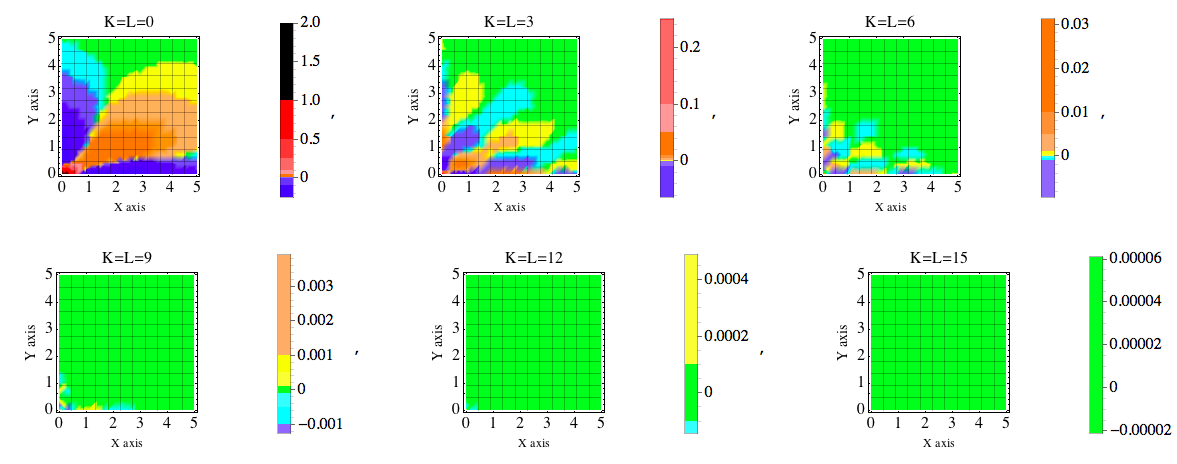
\includegraphics[width=16cm]{Chapitre5/GraphPDFGDBVEPolynomial.png}
			\caption{Error map for the joint PDF of a $DBVE(1/2,2,1/4)$ distribution approximated by polynomial expansion}\label{DBVEPDFPolynomialExpansion}
		\end{center}
	\end{figure}
\end{center}
An acceptable level of error is reached at almost every point of the bivariate probability density function with an order of truncation equal to $5$. Figure \ref{DBVEPDFMnats} shows the approximation error of the moment-recovered based method. Increasing values of $\alpha$ and $\alpha\rq{}$ are considered. 
\begin{center}
	\begin{figure}[!h]
		\begin{center}
			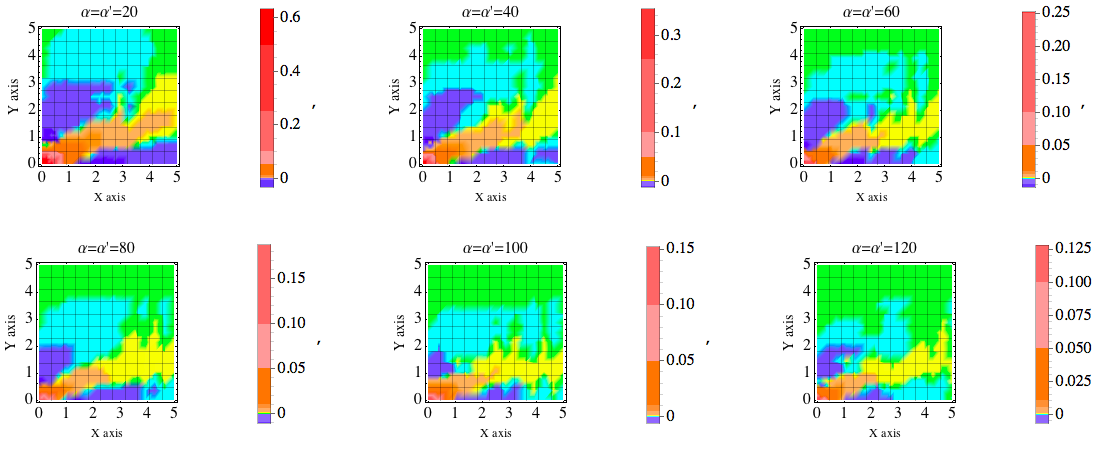
\includegraphics[width=16cm]{Chapitre5/GraphPDFGDBEVEMnats.png}
			\caption{Error map for the joint PDF of a $DBVE(1/2,2,1/4)$ distribution approximated by the moment-recovered method}\label{DBVEPDFMnats}
		\end{center}
	\end{figure}
\end{center}
The approximation of the moment-recovered based method works quite well too. However, the polynomial expansion seeems to be better suited to the problem due to the geometrical decay of the coefficients of the expansion. In order to provide a fair comparison, we perform an approximation of the Marshall-Olkin bivariate exponential distribution in the next subsection. 
\subsubsection{The Marshall-Olkin bivariate exponential distribution}
The Marshall-Olkin bivariate exponential distribution - $MOBVE(\lambda_{1},\lambda_{2},\lambda_{12})$ has been introduced in \citet{MaOl67} with reliability interpretations. It aims at modelling the time-to-failure of a two components system that receives shocks impacting one or both of the components. Each shock can cause the failure of none, one or both of the components. The definition implies the possibility that the two components fail at the same time, which means that the distribution admits a continuous and a singular part. This type of distribution might be pathological in a univariate context but arises naturally within a two-dimensional framework. The Marshall-Olkin BiVariate Exponential distribution $MOBVE(\lambda_{1},\lambda_{2},\lambda_{12})$ has been originally characterized through its joint survival function
\begin{equation}\label{MOBVEJointSurvival}
\overline{F_{X,Y}}(x,y)=exp(-\lambda_{1}x-\lambda_{2}y-\lambda_{12}max(x,y)).
\end{equation}
The BPDF associated with this distribution is divided into the sum of an absolutely continuous part with respect to the bivariate Lebesgue measure and another part being singular, defined on the line $\{x=y\}$. The BPDF can be written as
\begin{eqnarray}\label{MOBVEJointPDF}
f_{X,Y}(x,y)&=&\lambda_{2}(\lambda_{1}+\lambda_{12})\overline{F_{X,Y}}(x,y)\mathbf{1}_{x>y}(x,y)\label{MOBVEContinuousPart1}\\
&+&\lambda_{1}(\lambda_{2}+\lambda_{12})\overline{F_{X,Y}}(x,y)\mathbf{1}_{x<y}(x,y)\label{MOBVEContinuousPart2}\\
&+&\lambda_{12}e^{-\lambda max(x,y)}\mathbf{1}_{x=y}(x,y)\label{MOBVESingularPart},
\end{eqnarray}
where $\lambda=\lambda_{1}+\lambda_{2}+\lambda_{12}$. The Laplace transform associated to the  MOBVE distribution is 
\begin{equation}\label{MOBVELaplaceTransform}
\widehat{f_{X,Y}}(s_{1},s_{2})=\frac{(\lambda-s_{1}-s_{2})(\lambda_{1}+\lambda_{12})(\lambda_{2}+\lambda_{12})+s_{1}s_{2}\lambda_{12}}{(\lambda-s_{1}-s_{2})(\lambda_{1}+\lambda_{12}-s_{1})(\lambda_{2}+\lambda_{12}-s_{2})}.
\end{equation}
The distribution is not absolutely continuous with respect to the bivariate Lebesgue measure, the hypotheses of Proposition \ref{BivariateDensityExpansionTheo1} are not satisfied. However, we manage to isolate the singular part. So we can expand the defective probability density function associated with the continuous part of the distribution and add the singular part to the polynomial expansion in order to recover the entire distribution. The continuous part has a joint defective PDF $f_{X,Y}^{C}$, which is the sum of \eqref{MOBVEContinuousPart1} and \eqref{MOBVEContinuousPart2}, and admits a Laplace transform of the form
\begin{eqnarray}
\widehat{f_{X,Y}^{C}}(s_{1},s_{2})&=&\frac{s_{2} (\lambda_{1}+s_{1})}{(\lambda_{1}+\lambda_{2}+s_{1}) (\lambda_{1}+\lambda_{12}+\lambda_{2}+s_{1}+s_{2})}\\
&+&\frac{s_{1} (\lambda_{1}+s_{2})}{(\lambda_{1}+\lambda_{12}+s_{2}) (\lambda_{1}+\lambda_{12}+\lambda_{2}+s_{1}+s_{2})}.
\end{eqnarray}  
The generating function of the coefficients of the expansion is tedious, making it difficult to choose relevantly the parameters of the expansion. Unlike in the case of the DBVE distribution, we cannot ensure that the chosen parametrization is the best. Approximations with different parametrization are compared in terms of accuracy.
\begin{itemize}
\item \textbf{Parametrization 1:} $\{m_{1}=\frac{1}{\lambda_{1}+\lambda_{12}}, m_{2}=\frac{1}{\lambda_{2}+\lambda_{12}}, \nu_{1}=1, \nu_{2}=1\}$
\item \textbf{Parametrization 2:} $\{m_{1}=\frac{1}{\lambda_{1}}, m_{2}=\frac{1}{\lambda_{2}}, \nu_{1}=1, \nu_{2}=1\}$
\item \textbf{Parametrization 3:} $\{m_{1}=\frac{1}{\lambda}, m_{2}=\frac{1}{\lambda}, \nu_{1}=1, \nu_{2}=1\}$
\end{itemize}
We set $\{\lambda_{1}=1/2,\lambda_{2}=2,\lambda_{12}=1\}$.  In view of a future probabilistic application, the error on the joint survival function is very interesting. Let us see how the polynomial method performs when it comes to approximating the joint survival function. We also apply the moment recovered method with the inversion formula dedicated to survival function approximation. On Figure \ref{MOBVESurvivalApproxContinuousPart}, the relative difference between the exact value of the joint survival function and its polynomial approximation is plotted for different parametrizations. 
\begin{center}
	\begin{figure}[h!]
		\begin{center}
			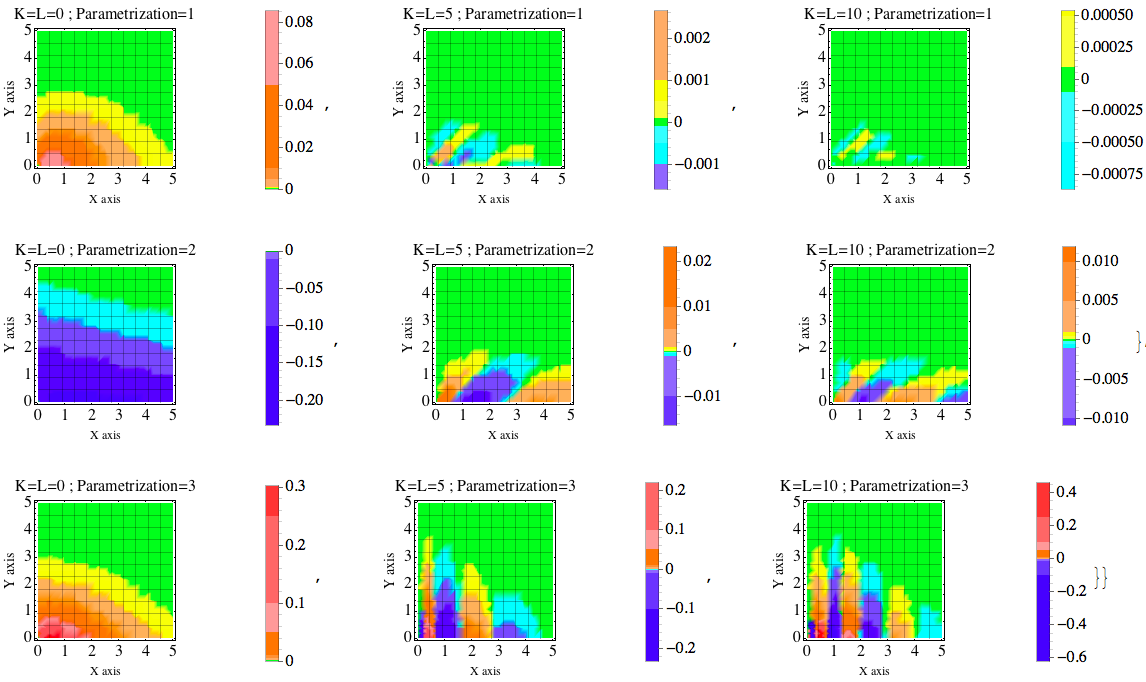
\includegraphics[width=16cm]{Chapitre5/GraphMOBVESurvivalPolynomial.png}
			\caption{Error map for the joint survival function of a $MOBVE(1/2,2,1)$ distribution approximated by polynomial expansion.}\label{MOBVESurvivalApproxContinuousPart}
		\end{center}
	\end{figure}
\end{center}
The first parametrization seems to be the most suited to the problem as the convergence towards the exact value is quicker. On Figure \ref{MOBVESurvivalMnats}, the difference between the exact value of the joint survival function and its moments approximation is plotted for increasing values of $\alpha$ and $\alpha'$.  
\begin{center}
	\begin{figure}[h!]
		\begin{center}
			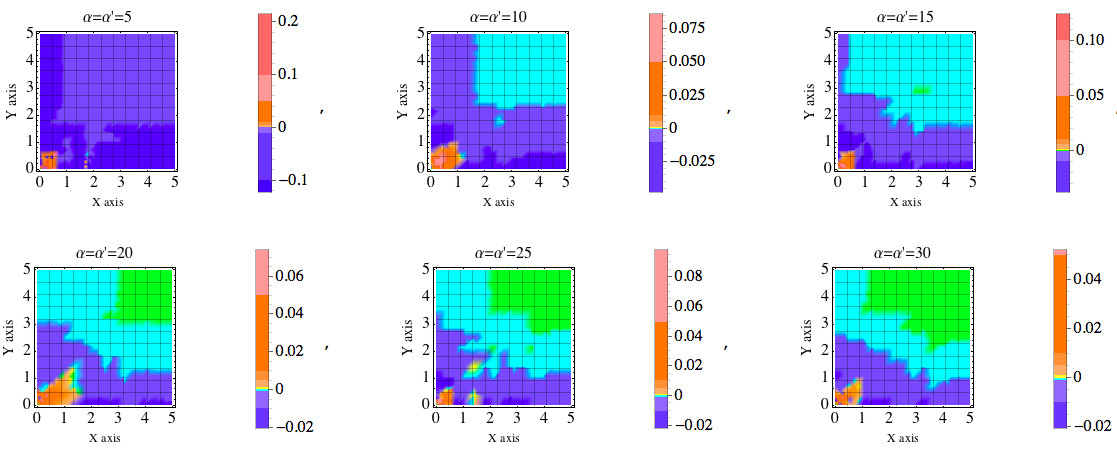
\includegraphics[width=16cm]{Chapitre5/GraphMOBVESurvivalMnats.png}
			\caption{Error map for the joint survival function of a $MOBVE(1/2,2,1)$ distribution approximated by the moment recovered method.}\label{MOBVESurvivalMnats}
		\end{center}
	\end{figure}
\end{center} 
The results are satisfying for both methods, even if it looks like the moment recovered method does not perform well for $x,y\in\left[0,0.5\right]$. One can note that the polynomial expansion with the first parametrization performs better than the moment-recovered based method. However, the moment-recovered based method has been enhanced in recent papers with the introduction of the scaled Laplace transform, see \citet{MnSa13,MnSaHa14}. These improvements have been made in the univariate case but might be extended soon to the multivariate case and comparison would be interesting in the future.  
\subsection{Approximation of the distribution of a bivariate claim amount distribution}\label{BivariateCompoundDistributionExpansion}
The main concern of this paper is to deal with the distribution of 
\begin{equation}\label{BivariateAggregateClaimWithCommonShock}
\left( \begin{array}{l}
Y_1 \\
Y_2 \end{array}
\right)  =
 \displaystyle\sum_{j=1}^{N}
\left( \begin{array}{l}
U_{1j} \\
U_{2j} \end{array}
\right).
\end{equation}
We assume here that the sequence of random vectors $(U_{1i},U_{2i})$ is \textbf{i.i.d.} and $DBVE(\mu_{1},\mu_{2},\rho)$-distributed. The number of claims is governed by a negative binomial distribution $NEG-BIN(a,p)$. In this case, the corresponding bivariate Laplace transform 
\begin{equation}\label{NegBinCompoundBivariateLaplaceTransform}
\widehat{g_{Y_{1},Y_{2}}}(s_{1},s_{2})=\left(\frac{1-p}{1-p\widehat{f_{U_{1},U_{2}}}(s_{1},s_{2})}\right)^{a}-(1-p)^{a},
\end{equation} 
exists if $\widehat{f_{U_{1},U_{2}}}(s_{1},s_{2})<p^{-1}$. In view of Corollary \ref{CorallaryParametrizationVersion2}, the parameters must be chosen under the constraints 
\begin{equation*}
\{m_{1}<2s_{1}^{*},m_{2}<2s_{2}^{*},r_{1}=r_{2}=1\},
\end{equation*}
where the couple $(s_{1}^{*}, s_{2}^{*})$ satisfies the equation $\widehat{f_{U_{1},U_{2}}}(s_{1}^{*},s_{2}^{*})=p^{-1}$. We set $\{\mu_{1}=1,\mu_{2}=1,\rho=1/4\}$ as parameters of the DBVE distribution and $\{a=1,p=3/4\}$ as parameters of the negative binomial distribution. In this particular case, if we set 
\begin{equation*}
\left\{m_{1}=\frac{1}{\mu_{1}(1-p)},m_{2}=\frac{1}{\mu_{2}(1-p)},r_{1}=1,r_{2}=1\right\}
\end{equation*}
as parameters of the reference distribution, the generating function of the coefficients of the expansion defined in \eqref{GenFunctionToLaplaceTransform} takes the form
\begin{equation}\label{CoefficientGeneraitingFunctionCompoundNegBINGDBVE}
B(z_{1},z_{2})=\frac{1}{1+z_{1}z_{2}(p^{2}-\rho(1-p)^{2}-p)}.
\end{equation}
The coefficients of the expansion are therefore $a_{kl}=(p^{2}-\rho(1-p)^{2}-p)^{k}\delta_{kl}$. The geometric decay of the coefficients implies a fast convergence of the approximation towards the desired function. It is easily checked that 
\begin{equation*}
\widehat{f_{U_{1},U_{2}}}\left(\frac{1}{2\mu_{1}(1-p)},\frac{1}{2\mu_{2}(1-p)}\right)<p, 
\end{equation*}
making the chosen parametrization valid. The exact value of the survival function is unknown. A benchmark value is derived through Monte Carlo simulations using algorithms described in \citet{60}. In order to get a good proxy via Monte-Carlo techniques, we produce $10^{5}$ realizations of the couple $(Y_{1},Y_{2})$. Figure \ref{NegBinCompoundDBVE} shows the difference between the values of the survival function derived by Monte-Carlo and by polynomial expansion. 
\begin{center}
	\begin{figure}[h!]
		\begin{center}
			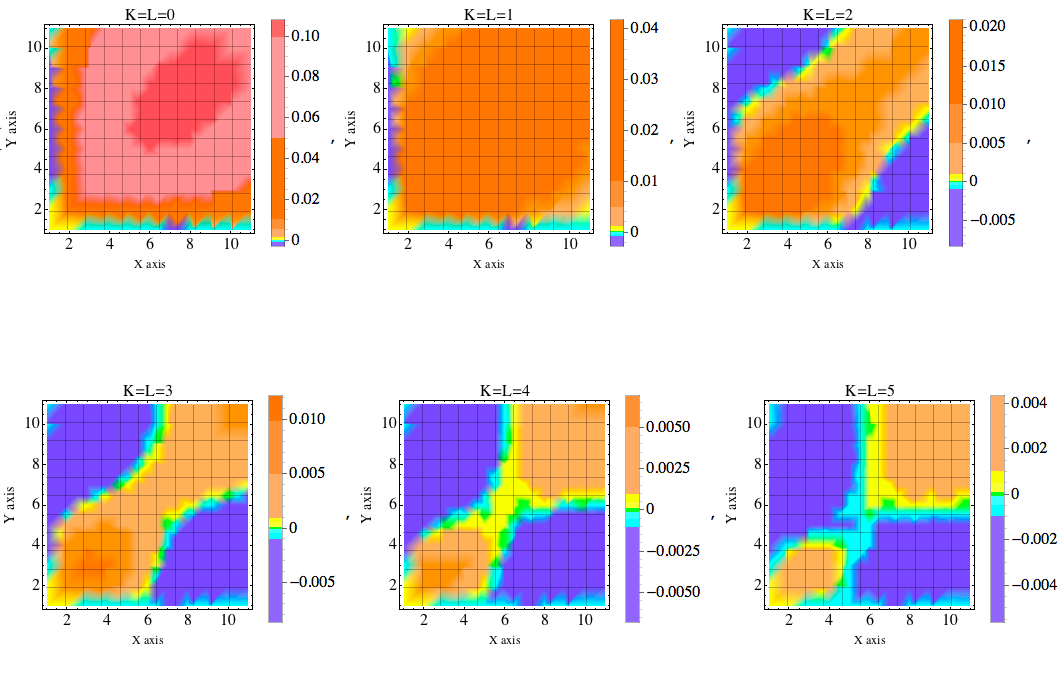
\includegraphics[width=12cm]{Chapitre5/GraphErrorSurvivalNegBinGDBVE.png}
			\caption{Discrete error map for the joint survival function of compound $NEG-BIN(1,3/4)$ $DBVE(1,1,1/4)$ distribution}\label{NegBinCompoundDBVE}
		\end{center}
	\end{figure}
\end{center}
One can see that we get close to the benchmark with an order of truncation equal to $5$. Figure \ref{3DPlotNegBinCompoundDBVE} provides a $3D$ visualization of the joint probability density and survival function of the distribution. 
\begin{center}
	\begin{figure}[h!]
		\begin{center}
			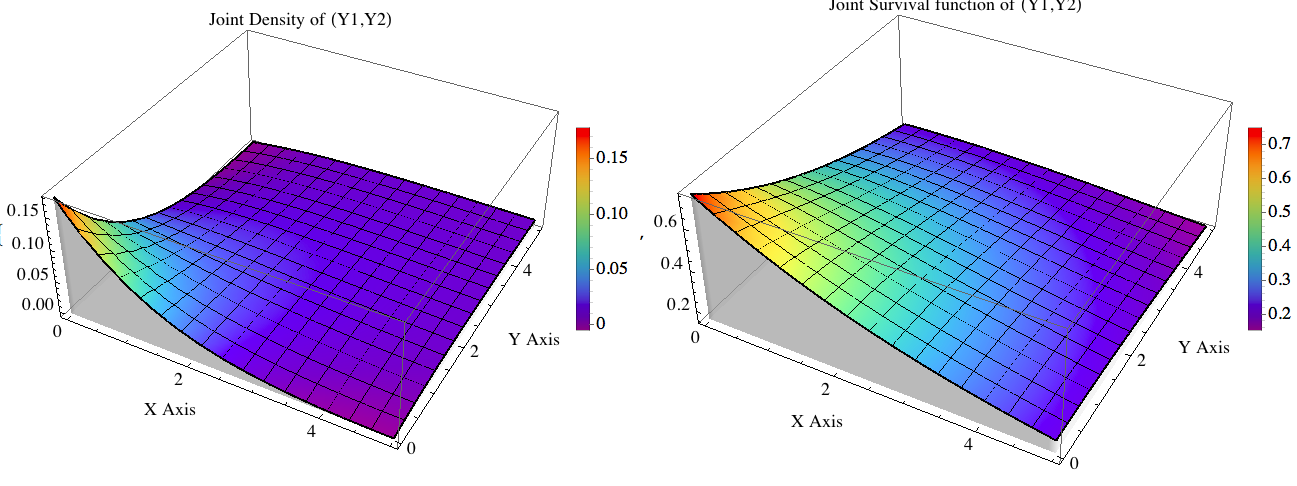
\includegraphics[width=12cm]{Chapitre5/Graph3DPDFSurvivalNegBinGDBVE.png}
			\caption{Joint survival function of compound $NEG-BIN(1,3/4)$ $DBVE(1,1,1/4)$ distribution with an order of truncation equal to $10$}\label{3DPlotNegBinCompoundDBVE}
		\end{center}
	\end{figure}
\end{center}
\subsection{Reinsurer's risk profile in presence of two correlated insurers}
We now consider a reinsurer with two customers. We assume that the reinsurer accepted a stop-loss reinsurance treaty with limit $b_{i}$ in excess of priority $c_{i}$ from insurer $i$, where $i=1,2$. This means that if $S_{i}$ is the aggregated claims amount for insurer $i$, then the reinsurer must pay $Z=min\left(\left[S_{1}-c_{1}\right]^{+},b_{1}\right)+min\left(\left[S_{2}-c_{2}\right]^{+},b_{2}\right)$. For risk management or pricing purposes, the reinsurer is interested in computing $P(Z>z)$ for different risk limits. To achieve that, one needs the joint distribution of $(S_{1},S_{2})$ and it is not enough to know the distribution of $(S_{1}+S_{2})$, which would often be easier to obtain.\\

As an illustration, we assume that each insurer has to pay some specific claim amount, which correspond to two independent components. We also take into account common shocks arising from events which cause claims for both insurers, like hail or storm episodes: for example, in the case of a hail episode, it might happen that $1$ windshield has to be replaced for insurer $1$ and that $2$ windshields have to be replaced for insurer $2$. Of course, for one particular event (the $k^{th}$ for instance) the two claims $U_{1,k}$ (incurred for insurer $1$) and $U_{2,k}$ (incurred for insurer $2$) are positively correlated, because they are influenced by the severity of the event causing the common shock.\\

We therefore consider that the vector $(S_{1},S_{2})$ is described as 
\begin{equation}\label{ReinsuranceModel}
\left( \begin{array}{l}
S_1 \\
S_2 \end{array}
\right)  =
 \displaystyle\sum_{j=1}^{N}
\left( \begin{array}{l}
U_{1j} \\
U_{2j} \end{array}
\right)
+
\displaystyle
\left( \begin{array}{l}
\sum_{i=1}^{N_{1}}V_{i} \\
\sum_{i=1}^{N_{2}}W_{i} \end{array}
\right).
\end{equation}
The first part of the right-hand side of \ref{ReinsuranceModel} is exactly the same as the random vector described in the introduction. The number of claims that incurs in the two portfolios is a counting random variable denoted by $N$. The severities of those claims are modeled through a sequence of \textbf{i.i.d} random vectors $\{(U_{1,j},U_{2,j})\}_{j\in\mathbb{N}}$ independent from $N$. The second part of the right-hand side of \ref{ReinsuranceModel} represents the claim amounts specific to each insurer. The numbers of claims are modeled by two independent counting random variables $N_{1}$ and $N_{2}$. The sequences $\{V_{i}\}_{i\in\mathbb{N}}$ and $\{W_{i}\}_{i\in\mathbb{N}}$ are formed by \textbf{i.i.d} nonnegative random variables that represent the claim sizes. These sequences are mutually independent and independent from $N_{1}$ and $N_{2}$. To recover the distribution of $(S_{1},S_{2})$ using the polynomial technology, we use the method described in this paper to the first part of right-hand side of \ref{ReinsuranceModel}. Regarding the second part, we may apply a univariate polynomial expansion to the two components separately. We have already presented the polynomial expansion in a univariate context in a previous work, we refer the reader to \citet{GoLoPo2014}. The joint probability density function of the second part is obtained by multiplying the marginal PDF due to the independence of the two components. The BPDF of $(S_{1},S_{2})$ is derived by convoluting the polynomial approximations of the different parts. One must pay attention to the singularities that arise from the non-zero probability of having $\{N=0\}$, $\{N_{1}=0\}$ and $\{N_{2}=0\}$.\\

For the common part, we assume that $N$ is governed by a negative binomial distribution $NEG-BIN(a,p)$ and that $(U_{1i},U_{2i}) $ is $DBVE(\mu_{1},\mu_{2},\rho)-$distributed. We set $\{a=1, p=3/4, \mu_{1}=1, \mu_{2}=1, \rho=1/4\}$. For the specific part, we assume that $N_{1}$ and $N_{2}$ are governed by negative binomial distributions with parameters $\{a_{1},p_{1}\}$ and $\{a_{2},p_{2}\}$, the claim sizes are Gamma distributed with respective parameters $\{\alpha_{1},\beta_{1}\}$ and $\{\alpha_{2},\beta_{2}\}$. We set $\{a_{1}=a_{2}=1, p_{1}=p_{2}=3/4,\alpha_{1}=\alpha_{2}=1, \beta_{1}=\beta_{2}=1\}$. To expand the common part, we set $\left\{m_{1}=\frac{1}{\mu_{1}(1-p)},m_{2}=\frac{1}{\mu_{2}(1-p)},r_{1}=1,r_{2}=1\right\}$ as parameters of the polynomial expansion in view of the good results obtained in Subsection \ref{BivariateCompoundDistributionExpansion}. The PDF of a geometric compound distribution with exponential claim sizes is available in a closed form, so we do not need to use univariate polynomial expansions. In order to ensure the goodness of our method, we need benchmark values. A sample of $10^{5}$ Monte-Carlo simulations of $(S_{1},S_{2})$ is produced. On Figure \ref{NegBinCompoundDBVE}, the difference between the survival function obtained via Monte-Carlo and polynomial expansion is plotted. 
\begin{center}
	\begin{figure}[h!]
		\begin{center}
			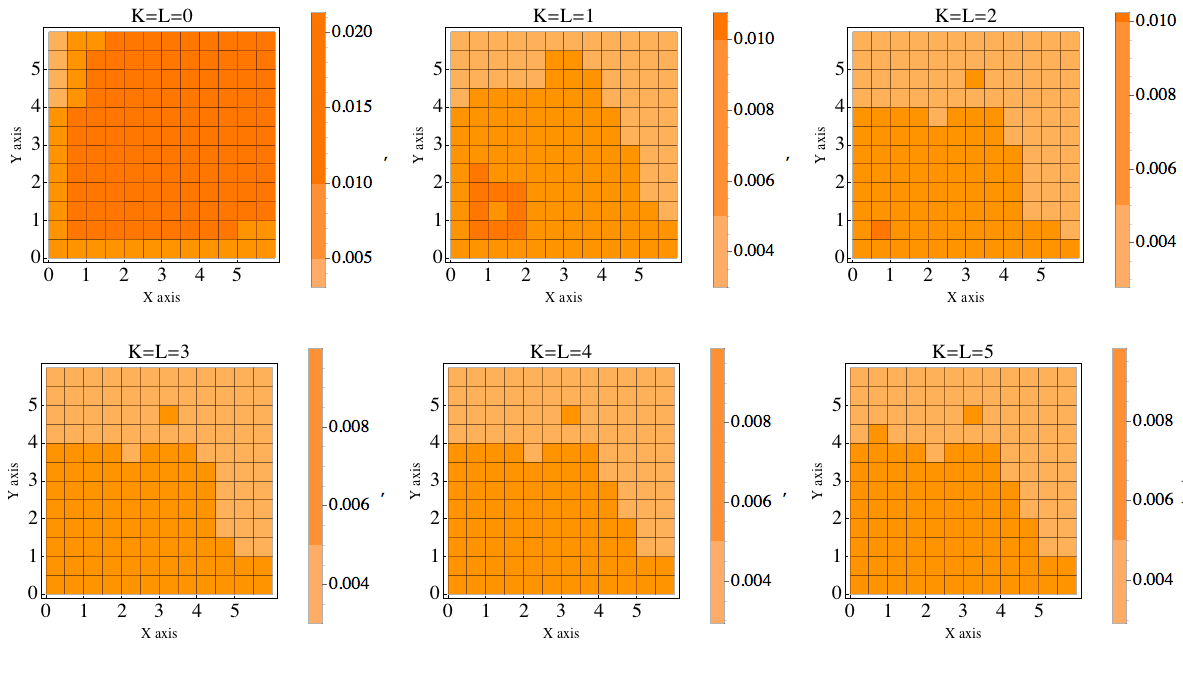
\includegraphics[width=14cm]{Chapitre5/GraphSurvivalFunctionAggregateClaim.png}
			\caption{Error map for the joint survival function of $(S_{1},S_{2})$ obtained by polynomial expansion}\label{NegBinCompoundDBVE}
		\end{center}
	\end{figure}
\end{center}
The level of error is still acceptable. Figure \ref{3DPlotReinsuranceApplication} displays the joint probability density and survival functions. 
\begin{center}
	\begin{figure}[h!]
		\begin{center}
			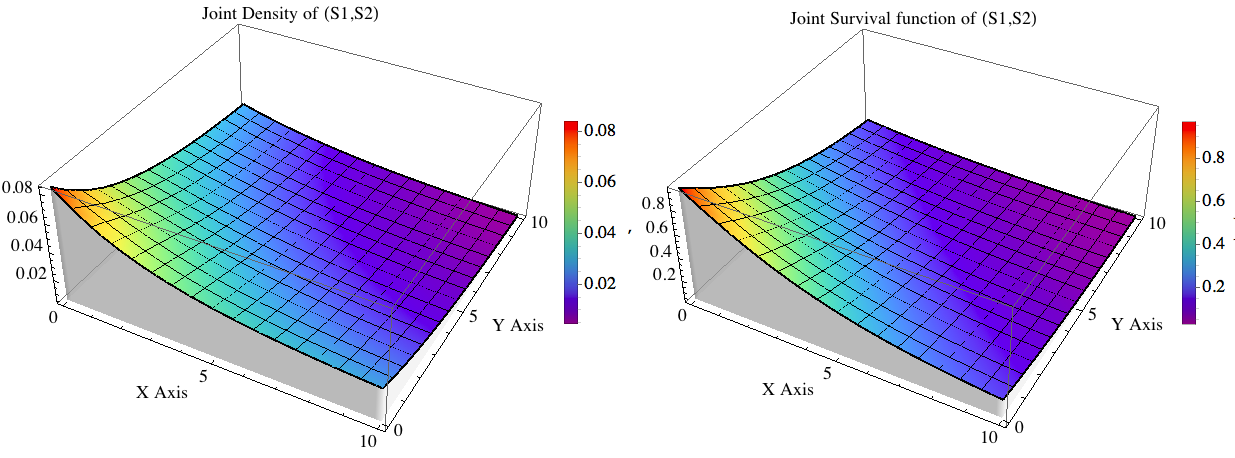
\includegraphics[width=16cm]{Chapitre5/Graph3DPDFSurvivalAggregateClaim.png}
			\caption{Joint density and survival function of the aggregate claims in the two insurance portfolios}\label{3DPlotReinsuranceApplication}
		\end{center}
	\end{figure}
\end{center}
As there exist a symmetry between the two portfolios, we assume that the same reinsurance treaty is proposed to the insurers with an equal priority and limit. We set $\{b_{1}=b_{2}=4, c_{1}=c_{2}=1\}$ . Recall that the reinsurance cost is modeled by a random variable defined as 
\begin{equation}\label{ReinsuranceCostZ}
Z=min\left(\left[S_{1}-c_{1}\right]^{+},b_{1}\right)+min\left(\left[S_{2}-c_{2}\right]^{+},b_{2}\right).
\end{equation}
Figure \ref{ReinsuranceCostApplication} displays two graphics. On the left one, we plot the survival function of $Z$ delivered by the two methods. We can see that the two curves overlap. On the right one, we plot the difference between the two approximations to better appreciate their proximity. Some values of $P(Z>z)$ are given in Table \ref{ReinsuranceCostApplication}. 
\begin{center}
	\begin{figure}[h!]
		\begin{center}
			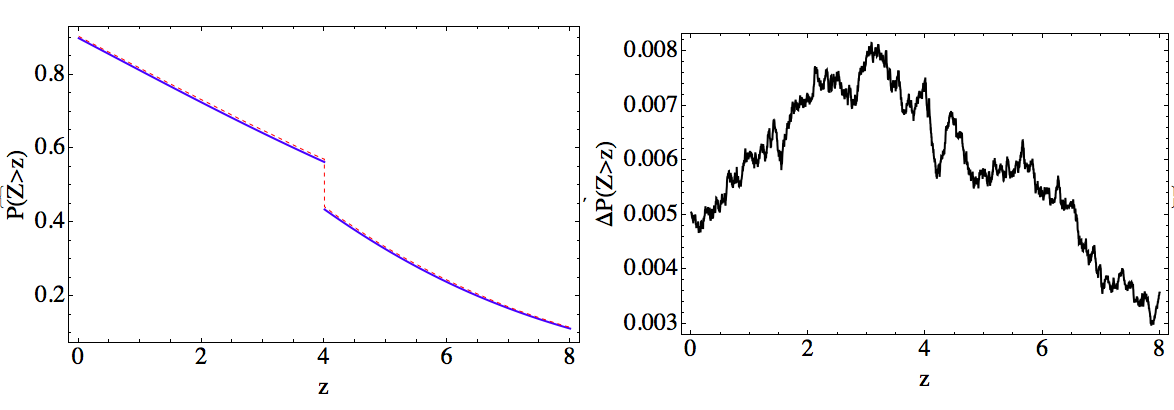
\includegraphics[width=14cm]{Chapitre5/GraphReinsuranceCost.png}
			\caption{Survival function of the reinsurance cost obtained by polynomial  expansion (blue) and Monte-Carlo simulations (red); Difference between the survival function obtained with Monte Carlo and the one obtained by polynomial expansion}\label{ReinsuranceCostApplication}
		\end{center}
	\end{figure}
\end{center}
\begin{center}
\begin{table}[h]
\begin{center}
\begin{tabular}{|c||c|c|}
\hline
&\multicolumn{2}{c|}{P(Z>z)}\\
\hline
z&Monte Carlo approximation&Polynomial approximation\\
\hline\hline
0 & 0.90385 & 0.898808 \\
 2 & 0.73193 & 0.724774 \\
 4 & 0.44237 & 0.435013 \\
 6 & 0.24296 & 0.237576 \\
 8 & 0. & 0. \\
\hline
\end{tabular}
\end{center}
\caption{Survival function of the reinsurance cost obtained by polynomial  expansion and Monte-Carlo simultions}\label{ReinsuranceCostApplication}
\end{table}
\end{center}
The results are quite promising. The polynomial expansion seems to be well-suited to carry out numerical calculations.  The operational advantage of numerical methods over Monte-Carlo techniques lies in the gain of computation time that they provide. It is difficult to quantify it as it varies given the software and the coding skills of the user. Note that, in the polynomial expansion case, the approximation of the PDF is almost immediate, although some computation time might be needed to derive survival function for instance.       
\section{Conclusion}
We have considered polynomial expansions of bivariate densities with well defined Laplace transforms. We focused our attention on densities on $\mathbb{R}^{+}\times\mathbb{R}^{+}$ and considered Laguerre polynomials expansions. MOBVE and DBVE distributions have been studied and numerical illustrations show great accuracy of the method. An application to a bivariate aggregate claims amount distribution with dependence has been proposed. This work is a numerical step that ensures the efficiency of the bivariate polynomial approach. Interesting applications follow from the fact that the approximants admit a tractable form. The approximation of the BPDF can turn into a nonparametric estimation of the BPDF. Indeed, the coefficients of the expansion can be replaced with their empirical counterparts when data are available. The statistical extension of this numerical method will be at the center of a forthcoming paper.  
\section*{Acknowledgements}
The authors would like to thank Pierre Miehe and Gilbert Macquart for their useful comments. This work is partially funded by the AXA research fund and the research chair \textit{Actuariat Durable}, sponsored by Milliman.

\bibliographystyle{francaissc}
\bibliography{Chapitre5/BiblioChap5}